\section{Results and Discussion}
System-level simulation was performed with representative AI inference workloads.

\subsection{Standby Power}
Migrating cold data and checkpoints to the FeRAM-backed tier yields more than 30\% reduction in standby power.
This reduction arises from suppressing periodic DRAM refresh for inactive regions.

\subsection{Resume Latency}
FeRAM allows direct restore of checkpoints without full DRAM wake-up.
Resume latency is reduced to the $\mu$s range, enabling near-instant resume after power gating and improving energy efficiency for mobile edge AI.

\subsection{Endurance}
FeRAM endurance of $10^{12}$~writes/year fits within FeRAM capability for checkpoint traffic.

% ===== Fig.2: Access time vs. retention(片段・HBM<FeRAM・右下凡例)=====
\begin{figure}[t]
\centering
\begin{tikzpicture}
\begin{loglogaxis}[
  width=\columnwidth, height=0.28\textheight,
  xmin=1, xmax=100, ymin=1, ymax=1e4,
  xlabel={Access time (ns)}, ylabel={Retention (s)},
  xtick={1,10,100}, ytick={1,10,100,1000,10000},
  grid=both, tick align=inside,
  legend style={draw=none, fill=white, at={(0.98,0.07)}, anchor=south east, font=\scriptsize},
  label style={font=\footnotesize}, tick label style={font=\footnotesize},
  clip=false
]

% HBM: red filled squares(常にFeRAMより下)
\addplot+[only marks, mark=square*, mark size=2.3pt, color=red, fill=red]
  coordinates {(1,1e0) (2,5e0) (5,2e1) (20,7e1) (100,3e2)};

% FeRAM: blue filled circles(各xでHBMより上)
\addplot+[only marks, mark=*, mark size=2.3pt, color=blue, fill=blue]
  coordinates {(1,1e1) (2,1e2) (5,6e2) (20,2e3) (100,8e3)};

\legend{HBM DRAM (typ), FeRAM (typ)}
\end{loglogaxis}
\end{tikzpicture}
\vspace{-2mm}
\caption{Access time vs. retention. HBM: red filled squares; FeRAM: blue filled circles.
Axes: $10^0\!\sim\!10^2$ ns, $10^0\!\sim\!10^4$ s. Legend is inside (bottom-right).}
\label{fig:retention}
\end{figure}

\subsection{Implication of Results}
As shown in Fig.~\ref{fig:retention}, HBM provides the required access speed but suffers from volatility and limited retention.
FeRAM, by contrast, achieves orders-of-magnitude longer retention at comparable access times.
These results clearly indicate that FeRAM can compensate for the volatility weakness of HBM,
strengthening the case for hybrid HBM+FeRAM chiplet integration in mobile edge AI systems.
